\subsection{Real embeddings: displacement versus neighbourhoods}
\label{sec:real}

\begin{figure}[tbp]
  \centering
  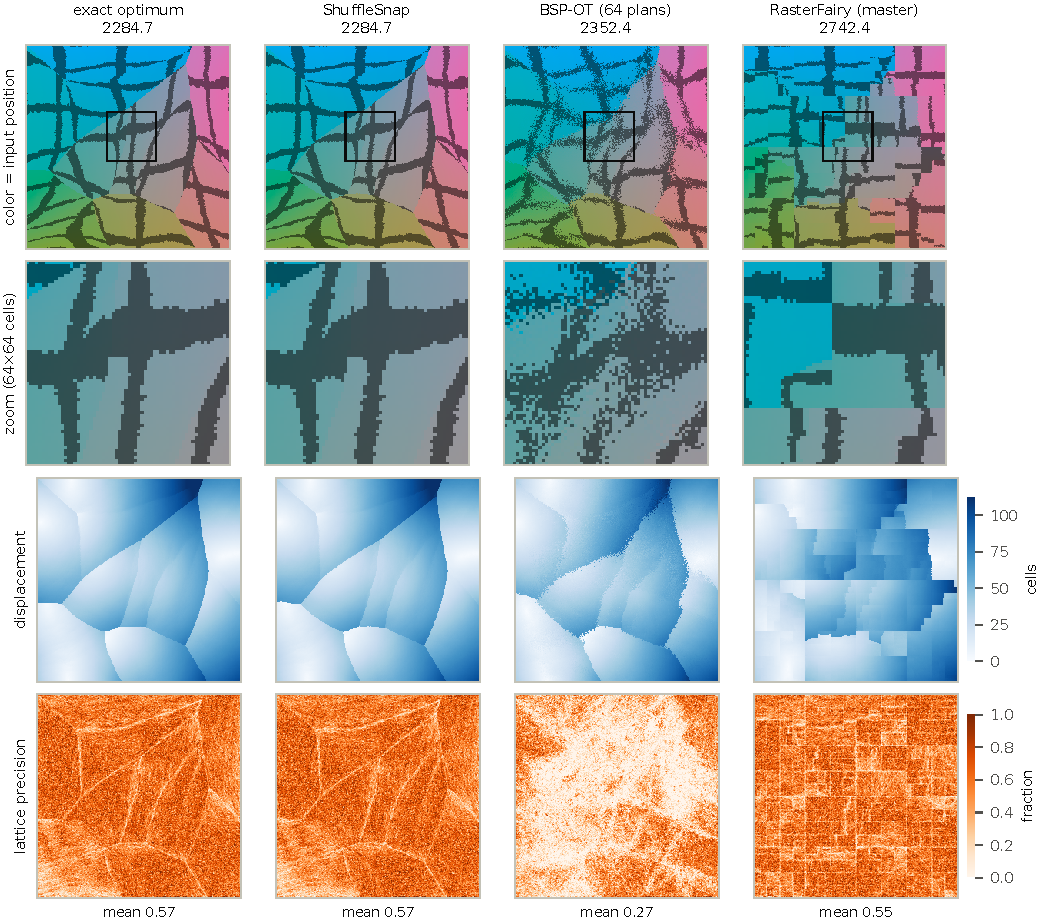
\includegraphics[width=\linewidth]{figures/fig_visual_mnist.pdf}
  \caption{All 70{,}000 MNIST digits, UMAP layout snapped to a $265\times265$ grid. Each
  point has the same color in every panel, set by its position in the input layout, and the
  dark bands are graph-paper lines drawn on the input, so bent lines show how a method
  deforms the layout, and color jumps or broken lines show where it tears it. The number under each method name is
  the mean squared displacement in cells$^2$. Row~2 enlarges the $64\times64$ box. Row~3
  shows each point's displacement. Row~4 shows the distance from each point's cell to its
  cell in the certified optimum (logarithmic scale; white means the optimal cell, so the
  optimum's own panel is blank). Row~5 shows lattice precision: the fraction of a
  point's occupied 8-neighbour cells whose points are among its 8 nearest input
  neighbours (higher is better). \ShuffleSnap\ is visually indistinguishable from the
  certified optimum: 74\% of its points sit on their optimal cell, and its few errors form
  the thin loops of one-cell shifts of Section~\ref{sec:anatomy}. BSP-OT is within 3\% of
  the optimal displacement, yet its median point is 8 cells from its optimal cell, and it
  halves lattice precision, because it scrambles local order (frayed lines and speckled
  boundaries in rows~1--2). RasterFairy's recursive slicing breaks the lines at rectangular seams.}
  \label{fig:visual}
\end{figure}

\begin{table}[tbp]
\centering\scriptsize
\setlength{\tabcolsep}{3.5pt}
\caption{Real embeddings, all 70{,}000 points (square exact-fit grid). Excess over the
certified optimum and neighbourhood measures are means over three method seeds; times are
medians on one thread (1T) and on 24 threads (24T, methods that use threads only). Memory is
the rise of peak resident memory during the call. kNN recall: fraction of each point's 10
nearest input neighbours among its 10 nearest grid neighbours. Lattice precision: fraction
of occupied 8-neighbour cells holding one of the point's 8 nearest input neighbours.}
\label{tab:real}
\resizebox{\linewidth}{!}{\begin{tabular}{llrrrrrrr}
\toprule
 & method & excess (\%) & mean sq. & time 1T (s) & time 24T (s) & mem (MiB) & kNN recall & lattice prec. \\
\midrule
MNIST UMAP & exact (certified) & 0 & 2284.7 & 82.0 & -- & 562 & 0.645 & 0.581 \\
 & ShuffleSnap fast & 0.031 & 2285.4 & 0.66 & 0.064 & 2 & 0.644 & 0.578 \\
 & ShuffleSnap balanced & 0.002 & 2284.7 & 2.27 & 0.16 & 2 & 0.645 & 0.580 \\
 & ShuffleSnap quality & $<$0.001 & 2284.7 & 7.03 & 0.54 & 2 & 0.644 & 0.580 \\
 & BSP-OT, 16 plans & 3.73 & 2370.0 & 0.49 & 0.088 & 16 & 0.305 & 0.255 \\
 & BSP-OT, 64 plans & 2.42 & 2340.0 & 1.98 & 0.28 & 42 & 0.305 & 0.249 \\
 & RasterFairy master & 20.0 & 2742.4 & 1.38 & -- & 42 & 0.631 & 0.551 \\
 & RasterFairy PyPI & 44.5 & 3301.0 & 11.2 & -- & 44 & 0.602 & 0.534 \\
 & bisection only & 34.4 & 3071.1 & 0.023 & -- & 0 & 0.569 & 0.498 \\
\addlinespace
Fashion UMAP & exact (certified) & 0 & 1802.6 & 76.0 & -- & 566 & 0.606 & 0.548 \\
 & ShuffleSnap fast & 0.008 & 1802.7 & 0.67 & 0.056 & 2 & 0.606 & 0.548 \\
 & ShuffleSnap balanced & 0.001 & 1802.6 & 2.31 & 0.17 & 2 & 0.607 & 0.547 \\
 & ShuffleSnap quality & $<$0.001 & 1802.6 & 7.23 & 0.56 & 2 & 0.607 & 0.547 \\
 & BSP-OT, 16 plans & 9.15 & 1967.5 & 0.50 & 0.088 & 16 & 0.295 & 0.245 \\
 & BSP-OT, 64 plans & 6.73 & 1923.8 & 1.98 & 0.28 & 42 & 0.334 & 0.275 \\
 & RasterFairy master & 24.6 & 2245.3 & 1.38 & -- & 42 & 0.611 & 0.532 \\
 & RasterFairy PyPI & 25.6 & 2264.5 & 11.1 & -- & 44 & 0.594 & 0.526 \\
 & bisection only & 23.0 & 2217.7 & 0.023 & -- & 0 & 0.544 & 0.477 \\
\bottomrule
\end{tabular}
}
\end{table}

Figure~\ref{fig:visual} and Table~\ref{tab:real} compare the methods on the full MNIST
and Fashion-MNIST embeddings. The default preset is within 0.002\% of the certified
optimum on both datasets, and the fast preset within 0.031\%. At about the same time as BSP-OT
with 16 plans (0.66\,s against 0.49\,s on one core), the fast preset is at 0.031\% and
0.008\%, where BSP-OT is at 3.7\% and 9.2\%.
In every panel their colour fields match the optimum's.

The two measures disagree on BSP-OT. With 64 plans, its displacement is only 2.4\% (MNIST) and
6.7\% (Fashion) above optimal, yet both neighbourhood measures fall to about half: kNN recall
0.31--0.33 against 0.61--0.65 for the optimum, and lattice precision 0.25--0.28 against
0.55--0.58. Averaged over plans, the merged BSP partitions are close to the transport
map, but they shuffle points locally. RasterFairy shows the opposite pattern: its
displacement is 20--25\% above optimal, yet its neighbourhood measures are close to the
optimum's. On Fashion-MNIST its kNN recall (0.611) even exceeds the optimum's (0.606),
because local order survives inside each slice and breaks only along the seams.
\ShuffleSnap's measures match the optimum's to within 0.003. Compared cell by cell with the
optimum (row~4, the figure's runs), \ShuffleSnap\ leaves 74\% (MNIST) and 69\% (Fashion)
of the points on their optimal cell and 93\% and 91\% within one cell, while BSP-OT's and
RasterFairy's median points are 8 and 19 cells from theirs on both embeddings. Even the optimum has lattice precision well below 1: an optimal transport map
from clustered data to a uniform grid tears the layout along cluster boundaries (the
white lines in row~5). Minimizing displacement and preserving neighbourhoods are
different objectives, and neither implies the other.
